\documentclass[12pt,twoside,notitlepage]{report}

\usepackage{a4}
\usepackage{verbatim}

\input{epsf}
\usepackage[pdftex]{graphicx}

\usepackage{listings}
\lstset{basicstyle=\scriptsize\ttfamily,breaklines=true,language={[Sharp]C}}

\raggedbottom                           % try to avoid widows and orphans
\sloppy
\clubpenalty1000%
\widowpenalty1000%

\addtolength{\oddsidemargin}{6mm}       % adjust margins
\addtolength{\evensidemargin}{-8mm}

\renewcommand{\baselinestretch}{1.1}    % adjust line spacing to make
                                        % more readable

\setcounter{secnumdepth}{2}				% make all subsubsections appear in the table of contents
\setcounter{tocdepth}{5}

\usepackage{parcolumns}

\begin{document}

\bibliographystyle{plain}


%%%%%%%%%%%%%%%%%%%%%%%%%%%%%%%%%%%%%%%%%%%%%%%%%%%%%%%%%%%%%%%%%%%%%%%%
% Title


\pagestyle{empty}

\hfill{\LARGE \bf David Barker}

\vspace*{60mm}
\begin{center}
\Huge
{\bf Functional Reactive Programming for Data Binding in C$\sharp$} \\
\vspace*{5mm}
Computer Science Tripos Part II \\
\vspace*{5mm}
Jesus College \\
\vspace*{5mm}
\today  % today's date
\end{center}

\cleardoublepage

%%%%%%%%%%%%%%%%%%%%%%%%%%%%%%%%%%%%%%%%%%%%%%%%%%%%%%%%%%%%%%%%%%%%%%%%%%%%%%
% Proforma, table of contents and list of figures

\setcounter{page}{1}
\pagenumbering{roman}
\pagestyle{plain}

\chapter*{Proforma}

{\large
\begin{tabular}{ll}
Name:               & \bf David Barker \\
College:            & \bf Jesus College \\
Project Title:      & \bf Functional Reactive Programming for \\
					& \bf Data Binding in C$\sharp$ \\
Examination:        & \bf Computer Science Tripos Part II \\
Word Count:         & \bf TBC \\
Project Originator: & Tomas Petricek \\
Supervisor:         & Tomas Petricek \\
\end{tabular}
}


\section*{Original Aims of the Project}

The project aimed to provide a general-purpose data binding framework for C$\sharp$ using concepts taken from functional reactive programming. Specifically, the goal was to implement a set of Haskell-style arrows and a binding framework which utilised these, and also to make invertible binding possible through the implementation of 'invertible arrows' -- a two-way extension of normal arrows. A secondary aim was to make the framework (and arrow implementation) as easy to use as possible, by making the syntax concise and readable, eliminating boilerplate code and allowing easy integration with the existing WPF data binding framework.

\section*{Work Completed}

All the original goals were met: a general-purpose data binding framework based on arrows has been implemented, and an extensive arrow implementation has been completed. As well as the standard operators, a series of more complex extra operators have also been added, and some additional arrow types have been included -- for instance, 'list arrows' which map between enumerable data types. The framework allows bindings in both directions, between multiple sources and multiple destinations, and the arrows can be used in conjunction with WPF data binding with reasonable ease.

%Continue this?

\section*{Special Difficulties}

None
 
\newpage
\section*{Declaration}

I, David Barker of Jesus College, being a candidate for Part II of
the Computer Science Tripos, hereby declare that this dissertation
and the work described in it are my own work, unaided except as may
be specified below, and that the dissertation does not contain
material that has already been used to any substantial extent for a
comparable purpose.

\bigskip
\leftline{Signed}

\medskip
\leftline{Date}

\cleardoublepage

\tableofcontents

\listoffigures

\newpage


%%%%%%%%%%%%%%%%%%%%%%%%%%%%%%%%%%%%%%%%%%%%%%%%%%%%%%%%%%%%%%%%%%%%%%%
% Chapters start here

\cleardoublepage

\setcounter{page}{1}
\pagenumbering{arabic}
\pagestyle{headings}


%%%%%%%%%%%%%%%%%%%%%%%%%%%%%%%%%%%%%%%%%%%%%%%%%%%%%%%%%%%%%%%%%%%%%%%
% Introduction

\chapter{Introduction}

It has become a firmly established practice when writing applications to separate the code managing the user interface from the business logic powering it. This is a key part of the principle of separation of concerns, and means that the interface can be safely changed without needing to modify the backend code (and vice versa, assuming the backend provides a consistent interface). Beginning with the traditional MVC architecture, this has led to the development of a family of system architectures such as MVPM and MVVM which enforce this principle.

\section{Data binding}

Data binding presents a mechanism for bridging the gap between the separated layers by allowing the developer to specify that some value in the user interface code should be bound to a property of the model. This usually simply means that whenever the value in the model changes, the data binding framework will ensure that the value in the user interface is also updated to the same value. However, bindings can often be more complex: for instance, there could be a text box in the user interface which reflects backend data but can also be used to change it (two-way binding). Alternatively, there might be a user interface component whose value is determined by some function of a variable in the model - consider a list view which displays a filtered and sorted version of a list stored in the model. There could even be values which depend on multiple sources, or more complex many-to-many bindings.

Many current languages and frameworks provide data binding features with varying levels of complexity. Java has a variety of extension libraries [examples] which allow the programmer to use data binding with Swing. Javascript too has a variety of possibilities, with a prominent example being the backbone.js MVC framework. Unfortunately, many of these are quite limited and difficult to use - backbone.js, for example, only provides one-way binding and requires a lot of boilerplate code from the programmer.

\section{Data binding in .NET}

Microsoft’s .NET framework offers a particularly powerful example of data binding through Windows Presentation Foundation (WPF). Based on the MVVM architecture, it has many features to allow things like two-way binding, binding through functions and bindings based on list operations. One of its key advantages is that the user interface can be defined entirely in XAML \footnote{Extensible Application Markup Language, an XML-based markup language for defining user interfaces and simple behaviour} with bindings being specified through XAML parameters. The view logic is then specified in the ViewModel which in turn communicates with the model. This means user interface designers can work purely in XAML without concern for the logic or binding mechanisms in place behind the scenes.

However, WPF suffers from a similar problem to many other data binding frameworks: advanced data bindings can be very complex and difficult to manage, and setting up bindings in the first place requires quite a lot of boilerplate code in the model and view. Furthermore, binding through functions requires special ‘value converter’ classes to be written. This is essentially an application of the Template pattern, and the value converters are not type safe - they take objects as input and return objects as output (and bindings with multiple inputs will simply take arrays of objects with no guarantee that the right number of values has been passed). [Maybe more disadvantages?] Clearly a more simple and general binding framework would definitely make application development simpler.

\section{Project inspirations}

Many useful ideas for data binding come from the area of functional programming. Functional reactive programming (FRP), for example, is a paradigm which nicely models the concept of data binding in a general way. Another useful concept is that of the `arrows' implemented in Haskell. An `arrow from type A to type B' essentially represents a process taking an input of type A and returning something of type B, and these can be arbitrarily combined in interesting ways to build up complex functions. More detail on both will be given in the next chapter.

The FRP paradigm was the inspiration for the project, which sought to implement a general-purpose data binding framework in C$\sharp$ using concepts derived from functional programming. I successfully implemented a framework which provides data binding in both directions, through arbitrary functions with arbitrary numbers of inputs and outputs, all with a simple syntax based on lambda expressions. Minimal boilerplate code is required to set up bindable properties - the containing class should extend \texttt{Bindable}, and from there marking arbitrary member variables and properties with the \texttt{[Bindable]} tag will make it possible to create bindings to and from them with a single function call. I also implemented a large variety of arrow types and arrow operators along with a number of utility functions to make creating and combining them simple.

\cleardoublepage


%%%%%%%%%%%%%%%%%%%%%%%%%%%%%%%%%%%%%%%%%%%%%%%%%%%%%%%%%%%%%%%%%%%%%%%
% Preparation

\chapter{Preparation}

\section{Background theory}

\subsection{Functional reactive programming}

Functional reactive programming (FRP) was one of the initial inspirations for the project. A good introduction is given by [http://conal.net/fran/tutorial.htm], which demonstrates how the principles can be applied to animation. In essence, functional reactive programming is a declarative way of specifying the relationships between different values. 'Signals' which change over time are created and passed around as first-class values, and other values can then be defined as functions of these signals.

One of the main advantages of FRP is that it removes the need for explicitly defining how values are to be kept consistent and writing code to make this so. This is clearly solving a very similar problem to data binding, and so inspired the idea of making data binding more like FRP.

\subsection{Arrows}

Arrows were introduced by Hughes as a generalisation of \texttt{monads}. A monad takes the form \texttt{m a}, representing some computation which will give a result of type \texttt{a}. These are often useful in representing sequences of operations and those which involve side-effects. The basic monad type interface provides an identity function, which gives a monad returning whatever its input was, and a means of chaining monadic functions together. One way of viewing these is as a way of letting the programmer chain together functions in a way controlled by the monad -- for instance, the monad could be written to ensure that some form of global state is passed through along with the function results, or it could be used to handle error conditions without the programmer needing to write extra code for this. In all cases it is essentially handling some side-effect or background operation for the programmer, allowing them to chain various operations together without explicitly handling the side-effects.

Arrows represent a generalisation of monads, in the sense that any monad can be equivalently implemented as an arrow. However, an arrow is of the form \texttt{arrow b c}, taking an input of type \texttt{b} and transforming it into an output of type \texttt{c}. The basic operators are similar: an \texttt{arr} operator takes a function as an argument and returns the arrow representing that function, and the \texttt{>>>} operator chains two arrows together such that the output of the first is passed through the second. Further to these, the \texttt{first} operator takes an \texttt{arrow b c} and returns an \texttt{arrow (b, d) (c, d)} -- an arrow taking a pair and applying the original arrow only to the first element of the pair. With these basic operators, a number of more complex standard operators can be built up. These are discussed in Section \ref{sec:simple_arrow_implementation} on the implementation of arrows.

Arrows were selected for this project as the semantic nature of an \texttt{arrow a b} is simply a transformation from an input of type \texttt{a} to an output of type \texttt{b}, an interpretation which works well as a generalised model of the nature of data binding.

\section{Requirements analysis}

From the outset, the main objectives of the project were to make the data binding framework syntactically clear and free from boilerplate, and to make the arrows as powerful and easy to use as possible. Therefore, some time was spent at the beginning of the project establishing what could be done to achieve this and just what sort of functionality would likely be needed.

To start off, I spent some time understanding how data binding is already done in .NET's WPF framework. It was clear that the existing approach involved a lot of repetitive coding from the programmer to set up bindable sources and destinations, and there were several different conflicting ways of actually creating the binding -- either in the XAML code describing the user interface or in the code-behind. Thus I decided a good first objective would be to find a way of making the framework completely general, with one consistent way of creating bindings which handles all the situation-specific details itself. I also focussed on ways of removing the usual boilerplate code for creating sources and destinations, replacing it with a base class which manages events and interactions and an attribute which can be placed on properties the programmer wishes to bind.

I also investigated what sort of features modern data binding frameworks implement, and which would be most useful for an arrow-based one. Binding through functions is not a new concept by any means, and indeed two-way binding is already implemented in .NET. However, in most cases these are fairly messy to set up -- in .NET, for instance, large \texttt{ValueConverter} classes have to be written to perform the transformation. It was decided that the cleanest way of handling this would be simply requiring that all bindings have an arrow attached. This way, the syntax is consistent whether the binding is direct or functional, and of course it is easy to pass in an identity arrow for a non-functional binding.

Exploring existing libraries highlighted a couple of extra features which I had not previously thought would be necessary: arbitrary many-to-many bindings, which are useful in a variety of situations, and list bindings. The latter refers to the situation where the data source is actually a list of data, and would have been possible with normal arrows. However, it would have been fairly messy to do, and simple tasks like filtering and mapping would have required large loops. Given list binding is done fairly often in practice, I decided it would make sense to add an arrow type for handling them and a variety of list processing methods.

For the arrows, the requirements were taken from the existing, successful implementation in Haskell. Essentially, I sought to implement all the main combinators and make the syntax as clear as possible. The main obstacle to keeping the syntax clean was the type system, and so much of the preparation time for arrows was spent devising the best approach for minimising type parameters and making the operators compatible. This stage of the project is described in greater detail in Section \ref{sec:arrows_overview}.

\section{Software engineering approach}

The implementation work was roughly done in two phases. In the early stages, a spiral model was used as it was unclear what the best way of implementing the arrows and binding framework would be. The first iteration was completed before the beginning of the project, and featured a very limited arrow class which worked on integers and supported only the basic combinators, and a binding framework which couldn't yet use arrows and required the sources and destinations to be special \texttt{BindingSource} and \texttt{BindingDestination} objects. Over several iterations the approach was refined until I found a suitable general and extensible implementation.

From there, development was issue-driven Agile with sprints defined to be the work packages designated at the start of the project (though many of these work packages were altered and expanded slightly). The FogBugz\footnote{\texttt{www.fogcreek.com/fogbugz}} issue tracker was used to manage this and keep track of the various milestones. The project was tested throughout development with a series of unit tests, and I frequently tried implementing complex data bindings to ensure that new features being added were compatible with what was already there and the syntax was still reasonably clean.

The entire project (dissertation included) was stored in a Git repository which was backed up on external storage and online with BitBucket\footnote{\texttt{www.bitbucket.org}}.

\cleardoublepage


%%%%%%%%%%%%%%%%%%%%%%%%%%%%%%%%%%%%%%%%%%%%%%%%%%%%%%%%%%%%%%%%%%%%%%%
% Implementation

\chapter{Implementation}

\section{Overview}

The implementation work consisted of two main parts: the arrows and the binding framework. As mentioned, these were both initially developed through repeated iterations as different strategies were being investigated and new options discovered. This chapter describes the main development work and highlights the various difficulties encountered along the way.


\section{Arrows}

\subsection{Overview} \label{sec:arrows_overview}

Implementing the highly functional idea of an arrow in C$\sharp$ posed an interesting challenge. Fundamentally, there were two main obstacles to overcome: C$\sharp$'s syntax, which is far clunkier than Haskell's; and the type system, which is far more restrictive and relies on static analysis at compile time. It was decided early on that arrows would be built on lambda expressions as these seemed the most natural way of expressing the desired functionality. C$\sharp$'s generic \texttt{Func<T1, T2>} type provided a good way of handling arbitrary lambda expressions between arbitrary types, and so this became the basis for the arrow type.

Tackling the type system was particularly difficult. I initially took the approach of writing arrow combinator functions so that they required no type parameters and instead inferred all their types by reflection. This made the syntax far neater and, using some run-time type checking, could plausibly be made type safe (though the compiler would have no way of enforcing it). However, after some experimenting it became clear that writing new operators and arrow types would be incredibly difficult using this approach, and the resulting code was very complicated and difficult to understand.

It was therefore decided that arrows and combinators should all be statically typed, as this would allow the compiler to do type checking and lead to much cleaner code. However, this meant the issue of the programmer having to provide long lists of type parameters to every combinator was still there. I was eventually able to solve this problem by writing the combinators in such a way that the compiler could always infer types from the arguments without the programmer needing to supply them. Several more situations were fixed by including static extension methods which would use the source object to infer some parameters, and a series of static helper methods were included in the class \texttt{Op} to help fill in the gaps. This was easier said than done in several cases (which will be discussed later), but ultimately I managed to eliminate type parameters completely from the syntax.

A further problem was how best to allow arrows from multiple inputs to multiple outputs. Simply having a \texttt{Func} with multiple inputs would not have worked as the arrow would have had to be rewritten for every given number of inputs, and to make matters worse \texttt{Func} is limited to one output. For some time I debated writing a generic binary-tree-structured type\footnote{All arrows work on nested pairs} to handle this, but on discovering C$\sharp$'s built-in \texttt{Tuple<T1, T2>} type I felt this would be the simplest option. This ended up complicating the data binding (as I will discuss later), but was entirely sufficient for supporting the arrow implementation.

%Maybe mention arrow intercompatibility?

\subsection{Simple arrows} \label{sec:simple_arrow_implementation}

The first objective in implementing arrows was to get the simple function-based arrow working, as all the others derive from this. As mentioned earlier, it was implemented using the C$\sharp$ \texttt{Func<A, B>} class to hold its function. An \texttt{Invoke} method is then exposed for using the arrow.

Whilst arrows can be constructed using \texttt{new Arrow<A, B>(function)}, a simpler syntax is provided by an extension method:

\begin{lstlisting}[language={[Sharp]C}]
var increment = ((int x) => x + 1).Arr();
\end{lstlisting}

\begin{figure}[!ht]
  \centering
  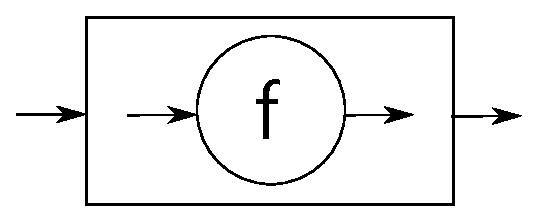
\includegraphics[width=50mm]{fig/ArrOperator.pdf}
  \caption{The Arr operator}
  \label{fig:arr_operator}
\end{figure}

The \texttt{Arr} operator effectively lifts a function to arrow status, in much the same way as the \texttt{arr} operator in Haskell. Arrow composition is also possible:

\begin{lstlisting}[language={[Sharp]C}]
var combinedArrow = arrow.Combine(anotherArrow);
\end{lstlisting}

\begin{figure}[!ht]
  \centering
  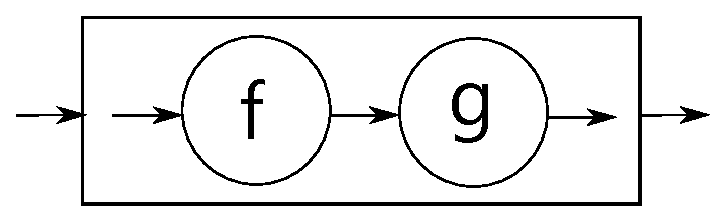
\includegraphics[width=50mm]{fig/CompositionOperator.pdf}
  \caption{The Combine operator}
  \label{fig:combine_operator}
\end{figure}

This is equivalent to \texttt{arrow >>> anotherArrow} in the Haskell syntax. Implementing a \texttt{>>>} operator was unfortunately not possible in C$\sharp$ as it does not allow user-defined operators. The \texttt{first} operator was then implemented to complete the basic arrow:

\begin{lstlisting}[language={[Sharp]C}]
var firstArrow = arrow.First(default(T));
\end{lstlisting}

Or, equally:\footnote{\texttt{Op} is the static class containing all arrow operators and extension methods}

\begin{lstlisting}[language={[Sharp]C}]
var firstArrow = Op.First(arrow, default(T))
\end{lstlisting}

\begin{figure}[!ht]
  \centering
  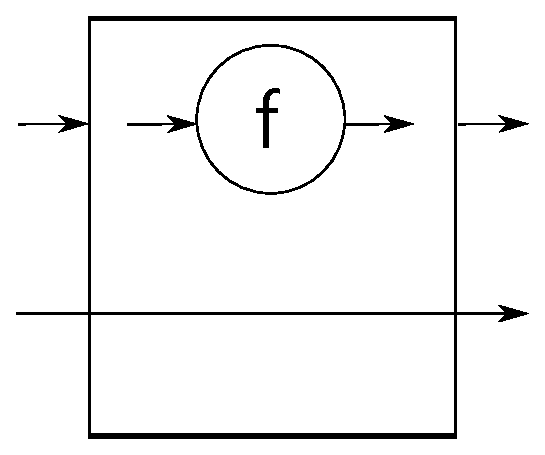
\includegraphics[width=50mm]{fig/FirstOperator.pdf}
  \caption{The First operator}
  \label{fig:first_operator}
\end{figure}

The above syntax may not immediately make sense. Essentially, the \texttt{default(T)} passes in null if \texttt{T} is a reference type and some sensible default if it is a null type. The only purpose for this parameter is to allow the compiler to infer the type of the second argument to the resulting arrow, and so any value of the appropriate type would work -- \texttt{default(T)} is used for simplicity. This is the one syntax `glitch' which I was unable to remove, and is explained in more detail at the end of this subsection.

Going beyond the basic operators, many composite operators were also implemented based on these simple combinators. For instance, \texttt{Second} was implemented in terms of \texttt{First}. The standard parallel combinator was also implemented as \texttt{And}:

\begin{lstlisting}[language={[Sharp]C}]
var parallelArrow = leftArrow.And(rightArrow);
\end{lstlisting}

\begin{figure}[!ht]
  \centering
  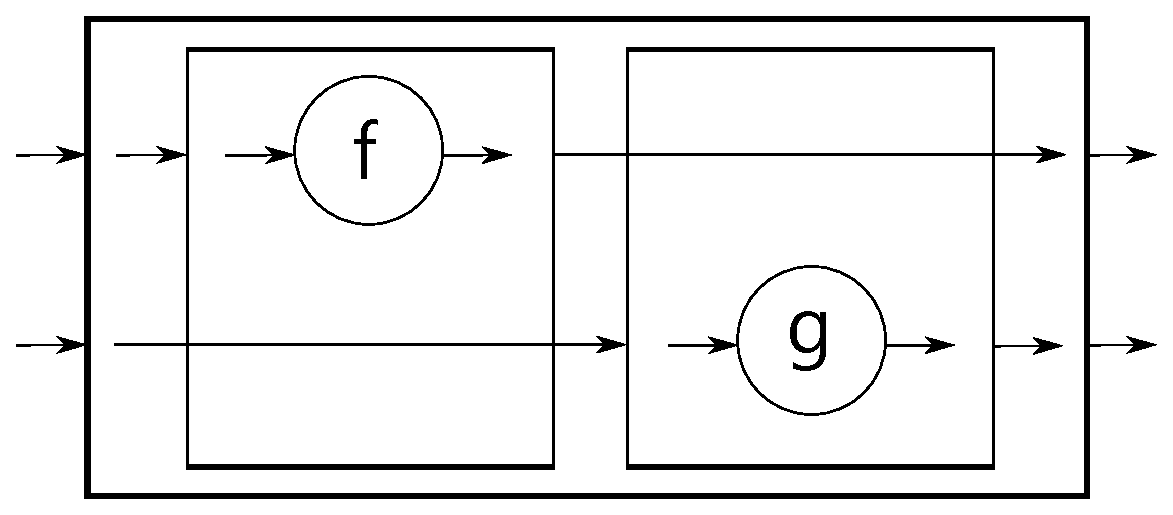
\includegraphics[width=50mm]{fig/AndOperator.pdf}
  \caption{The And operator}
  \label{fig:and_operator}
\end{figure}

This is equivalent to the \texttt{***} operator in Haskell, and executes the two arrows in parallel. This allows a number of complex operations to be conveniently parallelised in one arrow, which could likely be useful when working with data bindings between complex objects. The \texttt{Fanout} operator makes good use of this: given one input arrow of type \texttt{Arrow<A, B>} and two following arrows of types \texttt{Arrow<B, C>} and \texttt{Arrow<B, D>}\footnote{Note that the input types of the two arrows have to match the output type of the first arrow}, it returns an arrow which executes the input arrow, splits the result and then passes it through the two following arrows in parallel yielding a pair of results.

Given a pair result, it is then possible to recombine the two elements with a binary operator (passed as a \texttt{Func<A, B, C>}) using \texttt{Unsplit}. The following example recombines the tuple by adding its elements together:

\begin{lstlisting}[language={[Sharp]C}]
var unsplitArrow = arrowOnPairs.Unsplit((x, y) => x + y);
\end{lstlisting}

An example of a fairly elaborate composite operator is \texttt{LiftA2}. This essentially performs the same function as \texttt{Fanout}, but also takes a function for recombining the two results and so is effectively a \texttt{Fanout} arrow with an \texttt{Unsplit} operation at the end.

Figures~\ref{fig:arr_operator},~\ref{fig:combine_operator},~\ref{fig:first_operator} and~\ref{fig:and_operator} give a visual representation of some of the arrow operators, to make their effects more clear. A correspondence between Haskell arrow operators and the C$\sharp$ equivalents is given in Figure \ref{fig:operator_correspondence}.

%Include table showing correspondence between C$\sharp$ arrow operators and Haskell ones?

\begin{figure}
\centering
\begin{tabular}{| l | l |}
\hline
Haskell & C$\sharp$ \\
\hline
\texttt {arr f} & \texttt{f.Arr()} \\
\texttt{a >>> b} & \texttt{a.Combine(b)} \\
\texttt{first arrow} & \texttt{arrow.First(default(T))} \\
\texttt{second arrow} & \texttt{arrow.Second(default(T))} \\
\texttt{a *** b} & \texttt{a.And(b)} \\
\hline
\end{tabular}
\caption{Correspondence between Haskell and C$\sharp$ arrow operators}
\label{fig:operator_correspondence}
\end{figure}

\subsubsection{Challenges encountered} \label{sec:simple_arrow_challenges}

As mentioned in Section~\ref{sec:arrows_overview}, one of the main challenges in implementing usable arrows was eliminating the need for the programmer to specify large lists of type parameters when using arrow combinators. This was achieved by writing the combinators in such a way as to allow the compiler to infer the parameters, and in a few cases this required the use of extension methods (so that the type of the arrow it would be used with could be inferred).

The most difficult operator to implement cleanly was \texttt{First}. The problem here is that it takes an arrow from type \texttt{A} to type \texttt{B} and turns it into an arrow on tuples, applying the arrow to one input and leaving the other untouched. In Haskell, the type of the other input needn't be specified as the function doesn't make use of it. However, C$\sharp$'s type system is far more restrictive, and in constructing an arrow one must pass in the full types of its inputs and outputs. As a result, however the operator worked it would require the programmer to specify this third type.

The first implementation simply required the programmer to specify type parameters. However, there is no way in C$\sharp$ to specify the one unknown parameter and let the compiler infer the other two, and so the programmer would have to pass in all three types. This often became very unwieldy when the types of the original arrow were complex. For instance, consider the following example where an arrow from types \texttt{A} and \texttt{B} to types \texttt{C} and \texttt{D} is used with the First operator to allow an \texttt{int} to pass alongside as a third parameter:

\begin{lstlisting}[language={[Sharp]C}]
Arrow<Tuple<A, B>, Tuple<C, D>> originalArrow = [...];

var firstArrow = originalArrow
                         .First<Tuple<A, B>, Tuple<C, D>, int>();
\end{lstlisting}

It was decided that this was too cumbersome to be used in practice. The next attempt used a supplementary \texttt{First} method taking only the one unknown parameter, and using reflection to get the type of the arrow and invoke the original \texttt{First} method with its type. This works reasonably well and so was kept in the final version, but the code is incredibly messy due to all the reflection.

The final version was a modification of the first which allowed the compiler to infer the third type parameter by requiring that the user pass in a value of that type (hence the syntax shown in the last section). Although this isn't perfect, it is by far the cleanest workaround.

Another problem which was discovered was implementing standard polymorphic arrows, like an identity or one for swapping two inputs. This was also a result of the type system being too strict: to create an identity arrow, one had to specify in the definition what type it would work on. Several workarounds were considered for this, the most plausible being 'generic' arrows whose \texttt{Invoke} methods took a type parameter. However, the problem with this is that the resulting arrows would be very difficult to combine with non-generic arrows (and would most likely involve a lot of reflection). I eventually settled for implementing actual arrow subtypes for identity and other common functions, which take type parameters on construction -- these are discussed further in Section~\ref{sec:further_utility_arrows}.

\subsection{Invertible arrows}

At the time of writing the proposal, I was still unsure of the best way of implementing invertible arrows. There were two main strategies I was considering: simply requiring the user to supply an arrow for each direction, or providing a basic set of invertible functions and allowing the user to compose these together to build up more complex functions. The former wouldn't have worked very well as part of the advantage of using arrows in data binding is that simple ones can be re-used in building up multiple different bindings, and having to build up two arrows independently would be very messy and prone to error. The latter also has several problems. For instance, what functions should be made available to prevent the system being too restrictive? Also, if the functions were too simple then many would need to be combined in most cases, and this can cause a lot of unnecessary overhead (as explored in Section~\ref{sec:arrow_chaining_overhead}).

Ultimately, a solution roughly combining the two approaches was found. This was largely inspired by [REF], and is based on an \texttt{Arr} operator which takes \textit{two} functions rather than one -- one function for each direction. The arrows can then be combined using all the same combinators as are available for simple arrows (bar those which don't have inverses, such as \texttt{Unsplit}). As a result, it gives the same flexibility as allowing the user to simply define two arrows, but saves time by retaining the composability that makes arrows useful. An example of how an invertible arrow can be constructed using the \texttt{Arr} extension method is given below:

\begin{lstlisting}[language={[Sharp]C}]
var invertibleIncrement = new Func((int x) => x + 1)
                                .Arr((int x) => x - 1);
\end{lstlisting}

An invertible arrow can be used in the other direction by calling \texttt{Invert()} to get a new invertible arrow which is the original one reversed.

To make implementation simpler and reduce code duplication, many of the invertible arrow combinators make use of the standard arrow combinators in their implementations. The basic operators, \texttt{Arr}, \texttt{Combine} and \texttt{First}, are all overloaded so that any composite operators which use them will work for invertible arrows for free.

\subsection{List arrows}

Whilst exploring existing uses of data binding in WPF applications, it was discovered that a fairly common use case involves binding some form of list display to an enumerable data structure in the model. WPF provides support for this already, but trying to do it with arrows would be syntactically clunky -- for one thing, the arrow types would all be of the form \texttt{Arrow<IEnumerable<T1>, IEnumerable<T2>>}. To simplify this I decided it would make sense to implement an 'arrow on lists' abstracting away the actual list processing details and exposing a simple set of common list operators.

The result is a set of simple arrows implementing SQL-like functionality on enumerable data sources. List arrows are all of the type \texttt{ListArrow<T1, T2>}, which extends \texttt{Arrow<IEnumerable<T1>, IEnumerable<T2>>} for compatibility with existing arrows. There are a variety of simple list arrows which can be combined to build up complex functionality:

\begin{description}
	\item[\texttt{FilterArrow<A>}] Accepts a function from \texttt{A} to \texttt{bool}, which it uses to filter the list to those matching the predicate
	\item[\texttt{MapArrow<A, B>}] Accepts a function from \texttt{A} to \texttt{B} which it uses to map all items in the list to a list of \texttt{B}s
	\item[\texttt{OrderByArrow<A>}] Takes a function from two elements of type \texttt{A} to \texttt{int} and uses it to sort the list
	\item[\texttt{ReverseArrow<A>}] Simply reverses the input list
\end{description}

For simplicity, these arrows all essentially wrap Linq queries. As well as these operators, the standard functional operations \texttt{foldl} and \texttt{foldr} were implemented to make gathering a list into a single result easier.

The list arrows are all supported by a simple syntax which has been made possible using several extension methods. For instance, given a particular \texttt{ListArrow<int, int>}, one can quickly attach a filter to it as follows:

\begin{lstlisting}[language={[Sharp]C}]
var filtered = listArrow.Filter(x => x > 3);
\end{lstlisting}

In this example, the Filter extension method takes \texttt{listArrow} and the function \texttt{(int x) => x > 3}, creates a \texttt{FilterArrow<int>} out of the function, and returns a list arrow which is the original arrow and the filter arrow combined. Whole chains of list arrows can be quickly set up in this way:

\begin{lstlisting}[language={[Sharp]C}]
var listArrow = listArrow
                   .OrderBy((x, y) => y - x)
                   .Filter(x => x > 3)
                   .Map(x => "Number"+x)
                   .Reverse();
\end{lstlisting}

%More on foldl and foldr?

%\subsection{Choice arrows}

%\begin{itemize}
%	\item Not deeply implemented or tested but could be handy for some things, most likely convenient exception handling
%	\item This wouldn't be much good for bindings though
%\end{itemize}

\subsection{Further utility arrows} \label{sec:further_utility_arrows}

To simplify various common tasks, a number of simple utility arrows were written. These simply inherited from an arrow on the appropriate types, and initialised the arrow to some particular function in the constructor.

\begin{description}
	\item[Identity arrows] The identity arrow, though very rarely used in practice, plays a key part in several of the arrow laws. Creating it from a \texttt{Func} every time made the tests a lot messier, so a simple \texttt{IDArrow<T>} class was written which takes a type parameter and returns an identity arrow on that type. An invertible version of this was also written for the invertible arrow laws.
	\item[Swap arrow] This fulfilled a need which came up surprisingly often: given two types \texttt{A} and \texttt{B}, create an arrow on a \texttt{Tuple<A, B>} which swaps them around and outputs a \texttt{Tuple<B, A>}.
	\item[Tuple reassociation arrows] The tuple operations \texttt{assoc} and \texttt{cossa}\footnote{\texttt{assoc} takes a tuple ((a, b), c) and returns (a, (b, c)), whilst \texttt{cossa} does the opposite} turn up reasonably frequently in functional programming, and feature in several of the arrow laws. As these are fairly fiddly to implement I decided it would make sense to create utility arrows for both these functions.
\end{description}

%\subsection{Feedback in arrows}

%Discuss whether this would be useful or not, reasons for it not being there (lack of real-world use cases?) and how one might implement it.


\section{Data binding}

\subsection{Overall architecture}

The basis for the data binding system is a publish/subscribe network, where bound values publish events when they are updated and bindings update on receiving these events. A couple of alternatives were considered for this: the first idea was to have binding sources hold a reference to their target and a copy of the arrow associated with the binding, allowing them to simply update the referenced value via the arrow when needed. However, C$\sharp$ lacks the ability to hold references as member variables in this way. The simple approach of simply periodically polling all bound variables to check for updates was also considered, but this was clearly no good: polling is system-intensive and wasteful with many bindings using the same source, a binding target's value would potentially be 'invalid' between polling updates, and the bindings manager would need to store a copy of every bound variable.

Conveniently, C$\sharp$ provides simple syntax for event-based programming. Events can be created for a class and thrown with a method call, and other objects can subscribe and unsubscribe simply by adding or removing their handler methods from the event. The clearest approach was therefore to attach events to bindable objects and have them trigger whenever a bound variable is updated. The bindings manager, when creating a binding, need only tell the binding to subscribe to the source object's event and it will then be notified of all updates to variables. Information stored in the event arguments is used to filter out events from variables the binding is not watching, and the updated value is passed through the binding's arrow and then assigned to the destination variable. This approach is shown in Figure \ref{fig:binding_framework}.

\begin{figure}[!ht]
  \centering
  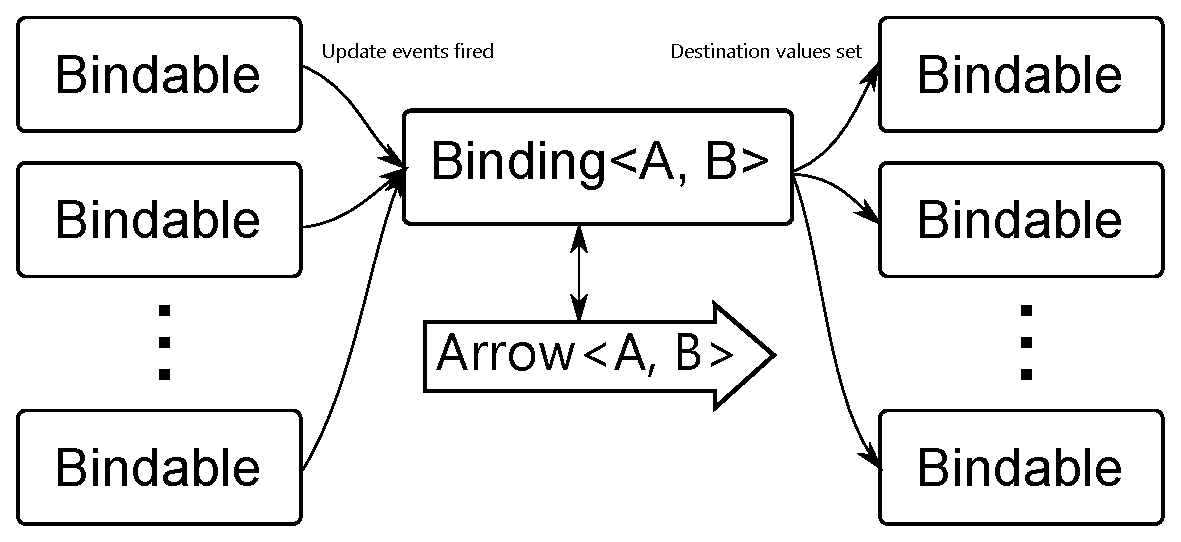
\includegraphics[width=\textwidth]{fig/BindingFramework.pdf}
  \caption{Overview of the binding method}
  \label{fig:binding_framework}
\end{figure}

An advantage of this technique is that sources and destinations can be treated in exactly the same way: both extend the \texttt{Bindable} base class, which handles events for binding updates and allows \texttt{Binding} objects to set the values of its bindable variables.

\subsection{Creating bindable sources and destinations}

One of the main problems with WPF data binding is the complexity of making sources 'bindable'. This usually requires that the programmer manually implement the \texttt{INotifyPropertyChanged} interface, creating appropriate events and overriding the set methods of all their properties such that they throw the right events. This often becomes a case of copying and pasting the code used for other data sources as it is almost always identical and includes boilerplate tasks like ensuring a variable's new value is different from its old one before throwing the event, and checking that the event isn't null.

For this project I decided to abstract these details away into a base class, called \texttt{Bindable}. This provides events for binding and a set of methods used by binding classes to manage data binding, many of which will be discussed later in this section. The most important are those which allow getting and setting of arbitrary variables by name using reflection, as these are the main interface used by the bindings manager. These have been designed to be dynamically type safe (that is, throwing exceptions at run time where type errors are encountered), to ensure the properties being accessed exist and to abstract away the differences between properties and simple public member variables\footnote{WPF does not allow binding to member variables, but for this project I decided there was no obvious need to distinguish between the two}.

The result of this is that instead of writing all the boilerplate code one would usually write, the programmer need only make their sources and destinations extend Bindable and all the usual things will be handled elsewhere leading to considerably less code clutter. A representative example of the final syntax is given in Listing \ref{lst:bindable_source_class}.

Another addition that can be seen in the listing is the \texttt{[Bindable]} attribute which has been used above the \texttt{value} property. This uses a PostSharp aspect, explained in the next section, to intercept the setter for throwing events and so relieve the programmer of having to do this themselves.

\begin{lstlisting}[language={[Sharp]C}, caption={Creating a bindable source class}, label=lst:bindable_source_class]
public class DataSource : Bindable
{
	[Bindable]
	public int value { get; set; }
}
\end{lstlisting}

\subsubsection*{PostSharp}

PostSharp is a C$\sharp$ extension which provides aspect-oriented programming (AOP) functionality. Essentially, AOP is a means of separating cross-cutting concerns from the code they affect, allowing 'aspects' to be written providing this common functionality. Markers can then be placed in the appropriate points, and the aspects will generate and inject their code into these locations at compile time.

In this case, the \texttt{Bindable} aspect will intercept the setter of any property or member variable it is placed above and insert code to check whether the value has changed and throw appropriate events if it has. This does not interfere with any setters the programmer may already have specified, as it defers to the programmer's setter before throwing the event for the value changing (thus ensuring the event is only thrown once all values are updated and any side-effects have occurred).

Unfortunately, the project budget only extended as far as the free version of PostSharp. Syntax for bindings could likely have been improved even further using the method and property introduction features provided by the full version, as this would have removed the need to extend Bindable. The unfortunate side-effect of the Bindable base class is that the class can no longer extend any other base class, as C$\sharp$ does not allow multiple class inheritance. However, in working with the binding framework it was found that this rarely caused problems that couldn't be worked around, and in any case patterns exist to overcome the lack of multiple inheritance in the general case\footnote{The 'composition over inheritance' pattern is one such technique which uses a shared base interface and a proxy object to 'inherit' from a class without using actual inheritance}.

\subsection{Creating bindings}

It was decided that it would make sense to manage all bindings in a given project centrally, so that constraints on cycles and conflicts can be enforced and bindings can be dynamically added and removed. Therefore, the \texttt{BindingsManager} class was implemented to create and maintain bindings. This is a static class handling all bindings for the project it is used in and exposing methods for creating and removing particular bindings. The programmer can call it passing in the sources, destinations and arrow they wish to use, and it will return a binding handle which they can use to remove the binding later if needed. The bindings manager also handles cycle and conflict detection, automatic creation of two-way bindings based on the arrow type and support for many-to-many bindings, all of which will be explained in this section.

\subsubsection{Syntax and usage}

In order to abstract away details like types and specific object references, the bindings manager operates on 'bind points' -- essentially, structures containing a reference to the \texttt{Bindable} source and a string representation of the property or member variable being bound. An extension method was written to make creating these simpler, as calling the constructor with the object and variable name turned out to make the overall syntax fairly cluttered. The standard way of making a bind point for an object 'obj' with property 'value' is thus \texttt{obj.GetBindPoint("value")}, which is a lot simpler to write.

Basic bindings (that is, from one source to one destination in one direction) can be set up by passing in a source bind point, and arrow to use for the binding and a destination bind point. An example of this is given in Listing~\ref{lst:creating_simple_binding}.

With the binding created, the bindings manager subscribes to the update event exposed by the \texttt{Bindable} base class and will thus be notified of any updates. The event is set up to contain the name of the property or variable which has changed so that multiple values from the same object can be bound to without any additional complexity, and as mentioned the \texttt{Bindable} class provides an interface allowing the bindings manager to freely access and modify those variables which have been marked as bindable. Although this largely precludes static type safety, dynamic type safety is provided wherever possible by using reflection to check that types match up and throwing explanatory exceptions where something has gone wrong.

\begin{lstlisting}[language={[Sharp]C}, caption={Creating a binding between two properties}, label=lst:creating_simple_binding]
BindingsManager.CreateBinding(
	source.GetBindPoint("value"),
	arrow,
	destination.GetBindPoint("result"));
\end{lstlisting}

\subsubsection{Two-way binding}

For simplicity, two-way bindings are inferred based on the type of arrow passed in; the function for creating bindings is overloaded such that passing in an invertible arrow will automatically set the binding up as two-directional. Two-way bindings are accomplished in much the same way as one-way ones, with the difference being that the binding subscribes to events from both sides and decides which way to update based on the binding point which triggered the update event.

The main difficulty encountered here was that these bindings initially led to infinite loops. If we consider a two-way binding between `A' and `B', whenever `A' is updated the binding will then update `B'. However, the setter for `B' has been modified to throw an event when it's updated signalling the binding to update, and so the binding is then forced to update `A' again. This continues back and forth in the main thread causing the whole application to hang.

The solution to this was to allow variables to be \textit{locked} when they are first updated. Essentially, the \texttt{Bindable} base class maintains a list of all the bindable variables it manages and holds a `locked' flag for each. Setting a variable through the methods supplied by \texttt{Bindable} will have no effect when the variable is locked, and so loops can be prevented simply by modifying the variable setter to lock, set and unlock the variable. Considering the previous example with this addition, when `A' changes it will first be locked and then set. `B' will then be updated by the binding, and will throw an event signalling the binding to update `A'. However, the binding's attempt to update `A' will fail and the loop will stop, unwinding back to `A' which is then unlocked.

\subsubsection{Cycle and conflict detection}

When setting up a large collection of arbitrary data bindings in a complex application, there is often the risk that some of the bindings could interfere with each other. This generally occurs in one of two ways:

\begin{itemize}
	\item A collection of bindings ends up forming a cycle, with every update to the first source property ultimately leading to an update of that same property
	\item One property is directly or indirectly bound to more than one source through functions which will not necessarily yield the same result
\end{itemize}

The first scenario is especially problematic for this binding framework as binding updates are performed in the same thread, so a binding cycle will lead to an infinite loop of updates causing the application to freeze. The second scenario doesn't necessarily break the application, but the resulting behaviour will be entirely unpredictable\footnote{This is because the order in which bindings are updated is governed by the order in which C$\sharp$ delivers events, and this is outwith the programmer's control}. Naturally, a useful data binding framework would need to handle these situations properly.

To tackle this problem, I implemented a \texttt{BindingGraph} class which is used by the \texttt{BindingsManager} and keeps track of the topology of all the existing bindings (leaving the details of actual bind points to the bindings manager). Whenever a new binding is added or an old binding is removed, the binding graph is notified and it updates its map of the bindings appropriately. It then provides methods which allow the bindings manager to query whether a new binding will introduce a cycle or conflict, and if so the bindings manager will know to abort the binding with an exception.

Both cycles and conflicts can be reduced to the same question: for each node in the binding graph, is there another node which is reachable from it via more than one path? Both situations are therefore handled by the same algorithm, which proceeds by depth-first searching from each node and maintaining a set of nodes which have been seen along the way. Rough pseudocode for this method is given in Listing~\ref{lst:cycle_conflict_pseudocode}.

\begin{lstlisting}[caption={Pseudocode for cycle and conflict detection}, label=lst:cycle_conflict_pseudocode]
for each node in the graph:
  seen = {}
  checkCycles(node, seen)

function checkCycles(node, seen)
  if node in seen:
    return 'cycle'
  else:
    add node to seen
    for each child node:
      checkCycles(child, seen)
\end{lstlisting}

Further to detecting these situations, another issue which had to be resolved was what action to take on finding a problem. Were the programmer to create a new binding between two objects which were already bound, a possible response would be to simply overwrite the old binding. This would prevent errors from the framework disrupting the user, and is also a fairly reasonable behaviour to expect. However, it was decided that this made the binding process too opaque and could lead to confusing behaviour if the programmer had accidentally overwritten a binding -- for instance, by mistyping the name of one of the objects they intended to bind. Therefore, whenever the programmer attempts to create a binding which would lead to a cycle or conflict, the framework throws an exception explaining the error. The behaviour of 'overwriting' an old binding is still possible as the \texttt{BindingsManager} provides a method for removing specific bindings, but now the programmer has to do the overwriting explicitly.

\subsubsection{Many-to-many bindings}

Many-to-many bindings presented an additional challenge for the binding system. It was decided that the best approach in terms of syntax would be to have the user pass in a list of source bind points, an arrow and a list of destination bind points, so as to mirror the syntax used in simple bindings. However, this simple approach is out of step with the way parameters are passed to arrows: by construction, all arrows taking multiple inputs will take them in the form of a binary-tree-structured Tuple\footnote{This can be verified by looking at the implementations of the operators; for instance, And converts two arrows (which may be on tuples) into an arrow on two-tuples containing the types of the original arrows, thus building up a binary tree structure}. As there didn't appear to be any C$\sharp$ syntax allowing the user to pass in binding sources in a similar fashion (such that the structure could be understood by the binding), it was decided that an argument marshaller/unmarshaller would be needed to handle the translation between lists of bind points and tree-structured tuples.

\begin{figure}[!ht]
  \centering
  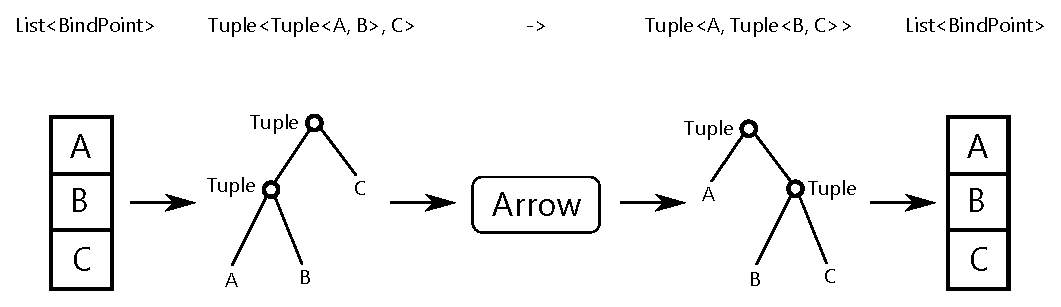
\includegraphics[width=\textwidth]{fig/ArgumentMarshalling.pdf}
  \caption{Marshalling a list of BindPoint sources to pass to an arrow and unmarshalling the result}
  \label{fig:argument_marshalling}
\end{figure}

By using reflection on the type of the arrow, I was able to convert a list of bind points to a binary-tree-structured Tuple. The code essentially does a recursive depth-first search through the input type of the arrow (obtained via reflection), simultaneously constructing a Tuple of the same structure and inserting values from the bind points wherever a 'leaf' is encountered in the type being searched. At the other end, a similar process is used to extract the values from the returned tuple and put them into a list which is then used to assign to the destination bind points. The process is illustrated in Figure~\ref{fig:argument_marshalling}, where a set of inputs of types A, B and C are being passed into an arrow from type \texttt{Tuple<Tuple<A, B>, C>} to type \texttt{Tuple<A, Tuple<B, C>>}.

\subsubsection{Problems encountered}

\paragraph{Type safety}

The binding framework at the moment is unfortunately not statically type safe: binding sources and destinations are of type \texttt{BindPoint}, which doesn't say anything about the actual type of the variable it refers to. An obvious solution would be to simply make the \texttt{BindPoint} class parameterised by the type of the variable it refers to (e.g. \texttt{BindPoint<int>} would refer to an integer variable), but this approach removed the ability to treat sets of bind points polymorphically which is used heavily by the methods for creating many-to-many bindings. As a result, it was decided that ensuring the types are correct should be left to the programmer. However, I was able to implement dynamic type checking at runtime so the framework will throw explanatory exceptions whenever the programmer has made a mistake rather than simply failing unexpectedly.

\paragraph{Binding to lists}

Unfortunately, the technique of intercepting assignments to trigger binding update events doesn't easily work for lists. The vast majority of list operations occurring in practice involve changing elements of the list rather than reassigning the list variable itself, and so the list's overridden assignment method will not be called. This means that list bindings will not update unless the programmer explicitly assigns a modified version of the list to itself:

\begin{lstlisting}[language={[Sharp]C}, caption={Explicitly reassigning a list to trigger a binding update}]
var tempList = listToBeUpdated;
tempList[3] = newValue;
listToBeUpdated = tempList;  // Triggers the binding update
\end{lstlisting}

This can be overcome by using an \texttt{ObservableCollection} instead of a list. An \texttt{ObservableCollection} is essentially the same as a normal list but provides a \texttt{CollectionChanged} event to which listeners can subscribe for notifications whenever the contents of the collection change, and so it would be fairly simple to have list bindings subscribe to these events and update in that way. However, this would require that all bound collections be of type \texttt{ObservableCollection} -- far more limiting than the current system which only requires that they be subtypes of \texttt{IEnumerable}, the base type of all collections.

\subsection{Integration work with WPF}

As the standard WPF binding method is fairly widely-used and naturally compatible with WPF, it was decided that arrows should be made compatible with it. WPF's standard approach to binding through a function is by creating a class extending the \texttt{IValueConverter} interface which implements the desired functionality through its \texttt{Convert} and \texttt{ConvertBack} methods. It was therefore reasonably simple to implement a value converter which allowed an arrow to be used for the conversion. However, this cannot be used when defining bindings in XAML as it does not allow constructor parameters to be passed in (it is possible to \textit{set} parameters in XAML, but this is a clunky workaround and the application would crash if the arrow was left unset). Creating WPF bindings with arrows is therefore limited to the code-behind.

One area where WPF integration went particularly well is in removing the boilerplate usually required to make a source bindable. In general, the programmer has to set up an event to be triggered when the bound variable changes and override the setters of all bound variables so that they throw this event. The method throwing the event also has to pass in the name of the variable triggering it (for disambiguation) and ensure that the event is not null (which occurs when it has no subscribers). This is usually combined with a method which stores variables' old values and checks that they have actually changed to avoid redundant updates. I was able to extract all this functionality into the \texttt{Bindable} base class and the PostSharp aspect, thus removing all the standard boilerplate. Variables can now be made bindable simply by making their class extend \texttt{Bindable} and placing the \texttt{[Bindable]} tag above them.

To demonstrate the WPF integration, a simple demo application was made in which a constantly incrementing 'time' variable is bound through a sin function to a progress bar. This is pictured in Figure \ref{fig:wpf_integration_demo}, and the main source code listings can be found in Appendix \ref{sec:wpf_integration_code}.

\begin{figure}[!ht]
  \centering
  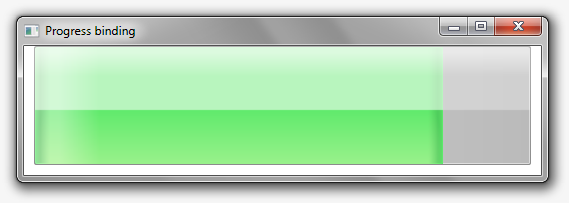
\includegraphics[width=\textwidth]{fig/WPFIntegrationDemo.png}
  \caption[WPF integration demo]{The WPF integration demo -- the progress bar goes sinusoidally up and down}
  \label{fig:wpf_integration_demo}
\end{figure}

\cleardoublepage


%%%%%%%%%%%%%%%%%%%%%%%%%%%%%%%%%%%%%%%%%%%%%%%%%%%%%%%%%%%%%%%%%%%%%%%
% Evaluation

\chapter{Evaluation}

\section{Correctness of arrow implementations}

The key requirement for an arrow type satisfying the original definition by Hughes is that it conforms to a set of 'arrow laws' defining how the various basic combinators should work. While there are numerous variations on the set of arrow laws, the standard ones used by Haskell are given in [REF]. These are listed in Appendix \ref{sec:arrow_laws}, along with their equivalent definitions using the C$\sharp$ syntax.

As invertible arrows conform to a slightly different set of arrow laws (which put extra requirements on their inverses), both one-way arrows and invertible arrows had to be tested separately. List and choice arrows were not separately tested as they are entirely built upon normal one-way arrows, and so will conform to the arrow laws for free if simple arrows do.

[Mention correctness proof by decomposition into lambda calculus?]

\subsection{Automated testing}

The main method of testing the arrow laws was using a set of unit tests, each testing one of the arrow laws using a large set of randomly-generated inputs. These were in most cases a simple case of generating the appropriate arrows for each side of the equality, pushing the set of inputs through both and checking that the outputs matched up. A few sample cases are given in the following subsections to illustrate the techniques used.

The tests are all supported by a large set of utility methods -- for instance, \texttt{AssertArrowsGiveSameOutput} and \texttt{AssertInvertibleArrowsGiveSameOutput} run the arrow comparison algorithms, whilst \texttt{AssertArrowEqualsFunc} checks that an arrow performs the same operation as a supplied C$\sharp$ \texttt{Func}.

\subsubsection{Simple arrows}

The laws for simple arrows can be found in Appendix \ref{sec:simle_arrow_laws}. The first few of these are fairly simple, but there were some which were more complicated to test -- indeed, the \texttt{SwapArrow} and \texttt{AssocArrow} arrows were mainly added to make these tests more readable and simpler to write.

One interesting case was the identity law -- in C$\sharp$ notation:

\begin{lstlisting}[mathescape]
new IDArrow<T>() $\approx$ id
\end{lstlisting}

This differs from the other laws because it has to be proven true over all \textit{types} rather than simply for all inputs. As such, the test proceeds by obtaining a representative list of types and using reflection to build an identity arrow for each, then uses the standard technique of firing lots or random inputs at it and asserting that the arrow does indeed represent the identity function. The set of types used was just the set of primitive types, obtained by querying the current assembly for all available types and filtering the non-primitive ones (as non-primitive types would have to be initialised to null, which defeats the purpose of testing correctness over all types).

To reduce complexity, 'random' arrows were produced by randomly selecting a function from a set of pre-defined functions and constructing an arrow with it. It seems reasonable to assume that if an arrow law were to hold for some combination of these functions, but fail on another, then the problem is more likely with the C$\sharp$ compiler than with the arrow implementation.

\subsubsection{Invertible arrows}

Invertible arrow laws are listed in Appendix \ref{sec:invertible_arrow_laws}, again with their C$\sharp$ equivalents. These were slightly more complicated to test than simple arrows as the laws have to hold for inverses as well.

[TBContinued]

\subsection{Correctness proof by decomposing into lambda calculus}

Explain the technique used to translate into lambda calculus and the likely correctness of this, and give a few sample proofs for some non-trivial arrow laws.

\section{Syntax evaluation}

\subsection{Arrow syntax}

Show major operators - arrow construction (niceish), arrow combination (niceish), First operator (not ideal - perhaps show all the differently imperfect ways of applying it); discuss the lack of type parameters despite the mad type-ing skillz going on (woo mad type inference skills!).

\subsubsection{Comparison with Haskell}

Firstly, mention difference in specifying lambdas and shizz (C sharp stunted from the start). From there, show how C sharp arrows create arrows from them (need types specified somewhere is an issue (no type inference like Haskell gets), C sharp also has a strict function calling syntax which doesn't allow Haskell's pretty currying syntax). Go on to give a few examples of complicated-ish arrows expressed in both? Also, maaaybe mention the shiny new syntax Haskell has for arrows, but the C sharp implementation can't really battle that so it's not worth going into much detail about.

\subsection{Binding syntax}

To evaluate how concise and readable the binding syntax is, a few case study applications were written using both normal WPF binding and arrow-based binding. The key code snippets from the resulting programs are listed in Appendix \ref{sec:case_studies}, and this section explores how the samples differ and how successful the attempt to simplify binding syntax and reduce boilerplate code was.

\subsubsection{Username two-way binding}

The first case study was relatively simple: given a data source containing a full name (forename and surname separated by a space), bind this information to two text boxes in the interface such that one shows the forename and the other shows the surname. To demonstrate that the binding was working, I also added a button which triggers a change in the name stored in the data source. A screenshot of the resulting application is given in Figure \ref{fig:case_study_name}, and code snippets are given in Appendix \ref{sec:case_study_name}.

\begin{figure}[!ht]
  \centering
  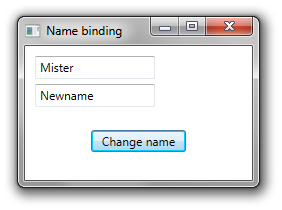
\includegraphics{fig/CaseStudyNameBinding.png}
  \caption{The username two-way binding application}
  \label{fig:case_study_name}
\end{figure}

This case study revealed a weakness in WPF's data binding, as it turned out to be impossible to do an invertible one-to-many binding linking the name data in the data source with the text box in the user interface\footnote{The IValueConverter interface's method for updating the reverse binding can take only one input, and so bindings have to be many-to-one}. It was possible to do the binding with two one-way bindings, one for each name, but reversing the binding -- taking the names, concatenating them and assigning this to the variable in the data source -- proved impossible without hacking around the inability to create invertible one-to-many bindings.

Looking at the code for creating the data source, it is clear that the arrow-based framework has considerably less boilerplate -- setting the name string up as bindable is a simple case of putting the \texttt{[Bindable]} tag above it, whereas the WPF approach involves creating an event, writing a method to throw that event if it exists and overriding the variable's setter to trigger that method. A real-world application would probably also have code to ensure the variable had actually changed value before calling the method.

Setting up the arrow is then a simple method call with two lambda functions defining the function either way, whilst the WPF version has two large \texttt{ValueConverter} classes for the forename and the surname. The arrow syntax is denser, however, which may make it harder to read -- it would perhaps be beneficial to allow invertible arrows to be constructed from two normal arrows so that the code can be more neatly separated.

For creating the actual binding, it's not clear which is better. The arrow-based code is shorter, but also more complicated due to the need to construct arrays of sources and destinations. However, the comparison is not entirely fair -- the WPF code is simply creating two one-to-one bindings, and if the same was being done with the arrow code it would be a lot neater than it is as the bind points wouldn't need to be put into arrays.

\subsubsection{List binding from a mock database}

For a second case study, a simple `database' (a \texttt{List} of data for simplicity) containing information on orders placed for certain products was created. The objective for this was to bind this data to a list view, filtering it to only the orders with volume greater than one and mapping the result to a list of user-friendly strings describing the order (of the form ``Order from [name] in [location] for [volume] `[product]' from [supplier]''). The simple application is pictured in Figure \ref{fig:case_study_list}, and its source code is given in Appendix \ref{sec:case_study_list}.

%Should sort too?

\begin{figure}[!ht]
  \centering
  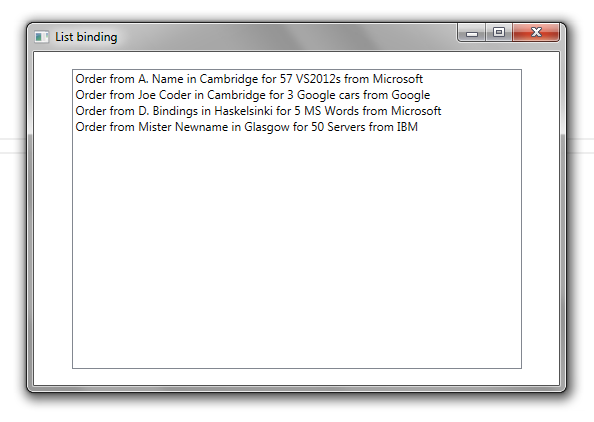
\includegraphics[width=\textwidth]{fig/CaseStudyListBinding.png}
  \caption{The list binding application}
  \label{fig:case_study_list}
\end{figure}

As with the last example, the arrow syntax is a lot more concise than the value converter. Filtering and mapping is done by calling \texttt{Filter} and \texttt{Map} on a base list arrow and passing in the appropriate lambda functions for each. The value converter, meanwhile, has to convert its input to the correct type and then manually cycle through each element, adding a string version of it to the result if its volume exceeds one. However, it could be argued that with more complex bindings like this the value converter is easier to debug than arrows: breakpoints can be conveniently set up inside the filtering loop and the code can be stepped through, whereas if the arrow gives unexpected results a lot of the work will be done by `behind the scenes' methods which the user cannot step through (this is more of an issue for list arrows as they are built up with the map, filter and sort operators).

The code for creating the binding is much simpler this time, and the arrow-based code is very short: only a single line calling the \texttt{GetBindPoint} methods of the source and destination and passing in the arrow. The WPF binding is again more verbose, requiring the programmer to create a new \texttt{Binding}; individually set the \texttt{Source}, \texttt{Path} and \texttt{Converter} properties\footnote{\texttt{Source} is the object to bind to, \texttt{Path} is the name of the property being bound and \texttt{Converter} is the \texttt{IValueConverter} used to convert the source value into the destination value} and attach it to the list view. The main advantage of arrow data binding here is the \texttt{GetBindPoint} method provided by \texttt{Bindable} objects, which simplifies specifying the bound variable to one call and means the variable name is `attached' to the object it belongs to.

\subsubsection{Some other demo}

Todo

\section{Performance testing}

\subsection{Arrow performance}

Naturally, the C$\sharp$ arrow implementation comes with some overhead. Being built on \texttt{Func} objects, arrows are slower than normal functions and slightly slower than plain \texttt{Func} objects. However, the difference isn't very large in most cases -- depending on how arrows are constructed, their performance is often very similar to using a plain \texttt{Func}. A number of performance tests were conducted to explore how using arrows affects performance, and the results are given in the next few sub-sections.

\subsubsection{Measuring technique}

A modular test framework was set up in which performance tests could be added by simply extending a base class and implementing methods for creating the arrow, the \texttt{Func} and the normal method. Timing was done by taking measurements of the total CPU time utilised by the current process, as follows:

\begin{lstlisting}[language={[sharp]C}]
TimeSpan start = Process.GetCurrentProcess().TotalProcessorTime;
RunTest();
TimeSpan end = Process.GetCurrentProcess().TotalProcessorTime;

double timeTaken = (end - start).TotalMilliseconds;
\end{lstlisting}

Each method was run for several million iterations and the resulting execution times were recorded and graphed to show relative performance.

\subsubsection{Simple function results}

To test how arrows perform implementing simple functions (on primitive types), a selection of simple arrows was implemented along with \texttt{Func} objects and normal functions implementing the same functionality. The functions chosen are given below, along with the number of iterations used for each\footnote{Different numbers of iterations were used to normalise the resulting graph}:

\begin{description}
	\item[Arctan] This function involved computing the \texttt{arctan} function on its input and converting the result to degrees. This was run for 5,000,000 iterations.
	\item[Quadratic] Computed the simple quadratic function $x^2 + 2x - 5$, and was run for 10,000,000 iterations.
	\item[Increment] Simply incremented its input, and was run for 10,000,000 iterations.
	\item[Pythagoras] Computed the function $\sqrt{2 x^2}$, as though finding the hypotenuse of a right-angled triangle with two sides of length $x$. For this one, the arrow was created by combining several sub-arrows, and so the overhead was considerably greater. 3,000,000 iterations were used here.
\end{description}

The results of these tests are given in Figure \ref{fig:simple_function_performance}. There are a few key observations which can be made here. Firstly, for simple functions like incrementing, arrows fare reasonably well with only slightly worsened performance. This is because these functions were implemented directly as one uncombined arrow, and so the overhead above a simple \texttt{Func} is minimal. Indeed, in the case of \texttt{arctan}, the performance difference is almost non-existent, as here function is sufficiently complex that the time taken to compute it becomes the main factor and makes the arrow overhead negligible. However, with the \texttt{Pythagoras} function, the arrow performs significantly worse than the other two. This is most likely due to the way the arrow is composed of many sub-arrows, as shown in the following code:

\begin{lstlisting}[language={[sharp]C}]
Func<int, int, int> add = ((int x, int y) => x + y);

arrow = Op.Arr((int x) => Tuple.Create(x * x, x * x))
          .Unsplit(add)
          .Combine(Op.Arr((int x) => (int)Math.Sqrt(x)));
\end{lstlisting}

Arrow chaining is the main performance issue arrows have, as increasingly complex combinations of arrows lead to a linear performance overhead. This issue is explored in more detail at the end of this sub-section. However, this is to be expected as a result of the implementation technique, and could perhaps be mitigated in future by optimising combined arrows as they are built up (discussed further in Section \ref{sec:performance_enhancements}).

\begin{figure}[!ht]
  \centering
  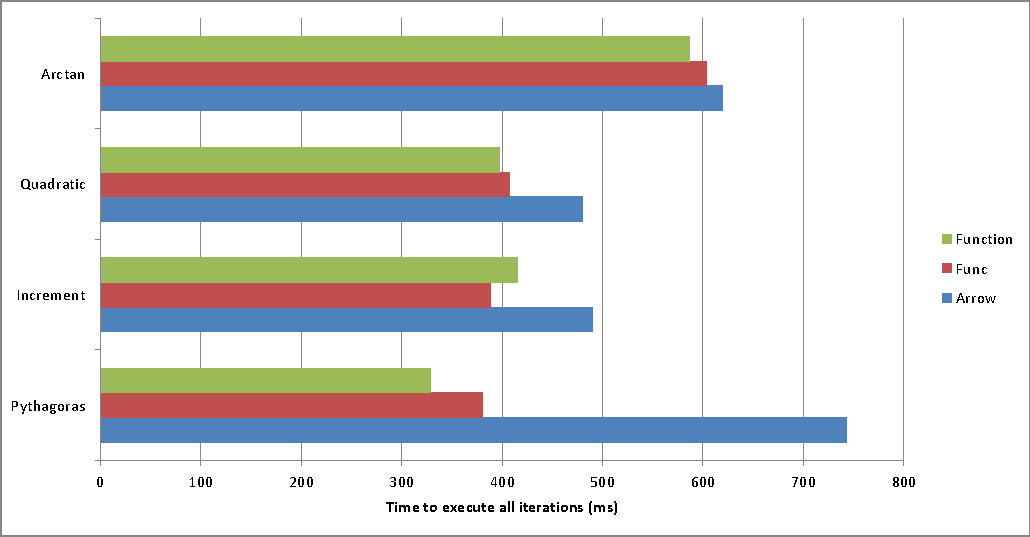
\includegraphics[width=\textwidth]{fig/SimpleFunctionPerformanceChart.pdf}
  \caption{Performance of arrows, Funcs and normal functions in implementing simple functionality}
  \label{fig:simple_function_performance}
\end{figure}

\subsubsection{List function results}

List arrows were also evaluated, this time in comparison with Linq queries and simple functions based on loops. For this, a simple mock database was created of \texttt{Person} objects, each having a name, age and reference to and \texttt{Employer} object. The three functions tested follow:

\begin{description}
	\item[Filter] The task here was to filter the input to the list of people over ten years old. This was run for 1,000,000 iterations.
	\item[Foldl] This tested the performance of the \texttt{foldl} method implemented for list arrows. The method had to combine all the \texttt{Person} objects into a single \texttt{Person} whose age was the sum of all the others and whose name was a concatenation of every name interspersed with `and' (``Alice and Bob and Eve and\ldots''). This was run for 300,000 iterations.
	\item[Order by then map] This function involved ordering the list by age and then mapping each person such that their name was followed by `` mapped''. This was also run for 300,000 iterations.
\end{description}

The results can be seen in Figure \ref{fig:list_function_performance}. Interestingly, arrows performed fairly well on the first two tests. The loop-based function was fastest for filtering, with arrows following close behind -- presumably as a result of their filter method also being a simple loop. The Linq expression was slowest as it seems the Linq overhead ended up dominating. For foldl, the results are too similar to draw much from, but the arrow implementation appears to have been slightly more efficient. Again, the difference is likely to have been influenced by the overhead associated with Linq queries. Finally, filter then map shows the effect of arrow concatenation slowing things down -- in the case of list arrows, this overhead is greater than normal because the \texttt{IEnumerable} is converted to a list before being passed on to the next arrow\footnote{This was necessary to make some of the list arrows compatible, as various type errors were being encountered previously}.

\begin{figure}[!ht]
  \centering
  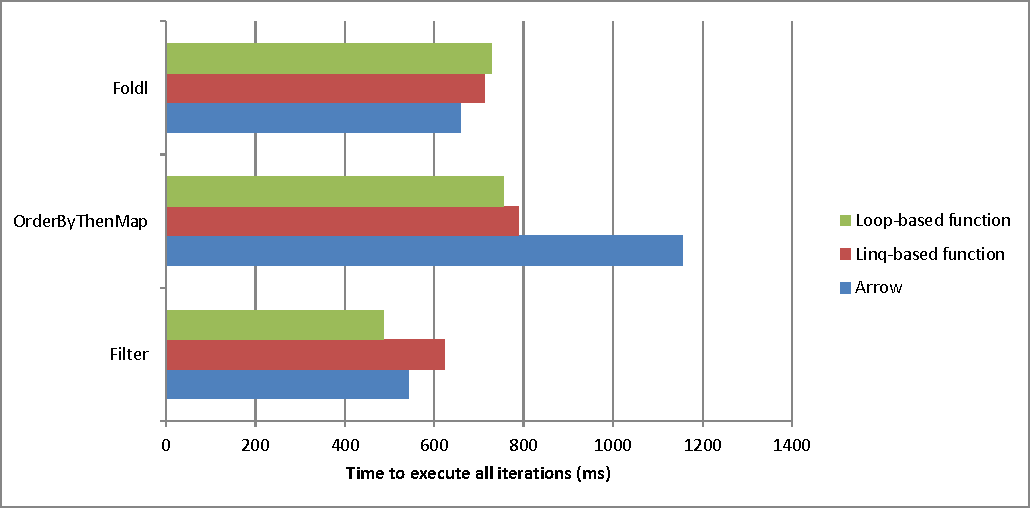
\includegraphics[width=\textwidth]{fig/ListFunctionPerformanceChart.pdf}
  \caption{Performance of arrows, Linq queries and normal (loop-based) functions in implementing simple list functionality}
  \label{fig:list_function_performance}
\end{figure}

\subsubsection{Overhead due to arrow chaining}
\label{sec:arrow_chaining_overhead}

As was discovered earlier on, complex arrow chaining imposes a performance overhead. To establish how severe the effects of this are, a test was set up in which the execution times of chains of identity arrows were compared. In an ideal world, fifty identity arrows chained end-to-end would run in the same time as a single one, but in reality the implementation leads to longer chains taking considerably longer to execute. A set of identity chains with lengths ranging from one to twenty was created, and each one was timed over 1,000,000 executions.

Fortunately, it was found that the execution time is linear in the length of the chain -- that is, each arrow combination adds only a constant extra overhead. The results can be seen in Figure \ref{fig:arrow_chaining_overhead}. Aside from small random variations, the timings clearly follow a linear trend. As noted earlier on, the overhead is far less pronounced when the function implemented is more complex than identity or incrementing, and so it is likely that for the majority of use cases combination overhead won't be significant enough to noticeably harm performance.

\begin{figure}[!ht]
  \centering
  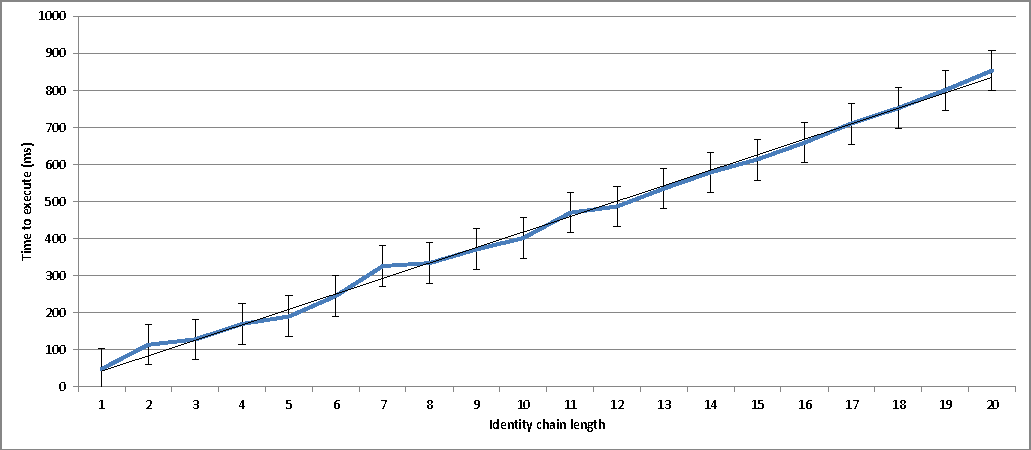
\includegraphics[width=\textwidth]{fig/IdentityChains.pdf}
  \caption{Execution times of chains of identity functions}
  \label{fig:arrow_chaining_overhead}
\end{figure}

\subsection{Binding performance}

Todo...

\cleardoublepage


%%%%%%%%%%%%%%%%%%%%%%%%%%%%%%%%%%%%%%%%%%%%%%%%%%%%%%%%%%%%%%%%%%%%%%%
% Conclusion

\chapter{Conclusion}

Conclusion goes here!

\section{Future work}

\begin{itemize}
	\item Performance issues - optimisations possible with dynamic expression trees?
	\item Messiness caused by use of Tuples - would be better with a custom tree type?
	\item Feedback arrows
	\item Better integration with WPF
	\item Syntax enhancements, perhaps through Roslyn
\end{itemize}

\subsection{Performance enhancements} \label{sec:performance_enhancements}

Blah

\cleardoublepage


%%%%%%%%%%%%%%%%%%%%%%%%%%%%%%%%%%%%%%%%%%%%%%%%%%%%%%%%%%%%%%%%%%%%%%%
% Appendices

\appendix

\chapter{Arrow laws} \label{sec:arrow_laws}

Here the arrow laws used in testing are presented both in Haskell syntax and as they were translated into C$\sharp$. For convenience, the following definitions are used:

\begin{lstlisting}
id = new Func<T, T>(x => x)
\end{lstlisting}

That is, id represents a C$\sharp$ identity function.

\begin{lstlisting}
first_f = new Func<Tuple<T, T>, Tuple<T, T>>(
  tuple => Tuple.Create(f(tuple.Item1), tuple.Item2))
\end{lstlisting}

This defines a \texttt{Func} which invokes a function 'f' on the first element of a tuple.

\section{Normal arrow laws} \label{sec:simle_arrow_laws}

\begin{samepage}
\begin{lstlisting}[mathescape]

Identity
arr id = id
new IDArrow<T>() $\approx$ id

Arr operator distributivity
arr (f >>> g) = arr f >>> arr g
Op.Arr(x => g(f(x))) $\approx$ Op.Arr(f) .Combine( Op.Arr(g) )

First operator distributivity
first (f >>> g) = first f >>> first g
f .Combine(g) .First<T>() $\approx$ f .First<T>() .Combine( g.First<T>() )

Associativity of arr and first operators
first (arr f) = arr (first f)
Op.Arr(f).First<T>() $\approx$ Op.Arr ( first_f )

Piping commutativity
first f >>> arr (id *** g) = arr (id *** g) >>> first f
f.First<T>() .Combine( id.And(g) ) $\approx$ id.And(g) .Combine( f.First<T>() )

Piping simplification
first f >>> arr fst = arr fst >>> f
f.First<T>() .Combine( Op.Arr(tuple => tuple.Item1) ) $\approx$ Op.Arr(tuple => Tuple.Item1) .Combine( f )

Piping reassociation
first (first f) >>> arr assoc = arr assoc >>> first f
f .First<T>() .First<T>() .Combine( new AssocArrow<T>() ) $\approx$ new AssocArrow<T>() .Combine( f .First<T>() )

\end{lstlisting}
\end{samepage}

\section{Invertible arrow laws} \label{sec:invertible_arrow_laws}

Todo

\cleardoublepage


\chapter{WPF integration demo -- code listings}  \label{sec:wpf_integration_code}

\section{Creating the bindable source}

\begin{lstlisting}
public class Time : Bindable
{
  [Bindable]
  public int CurrentTime { get; set; }

  private Timer timer;

  public Time()
  {
    CurrentTime = 0;
    // Make the CurrentTime variable increment every 25 milliseconds
    timer = new Timer(state => CurrentTime++, null, 25, 25);
  }
}
\end{lstlisting}

\section{The binding arrow}

\begin{lstlisting}
progressArrow = Op.Arr(
  (int x) => 50.0 + (50.0*Math.Sin(x / 30.0))
);
\end{lstlisting}

\section{Doing the binding}

\begin{lstlisting}
Binding binding = new Binding();
binding.Source = time;
binding.Path = new PropertyPath("CurrentTime");
// Make a value converter using the arrow
binding.Converter = new ArrowValueConverter(progressArrow);
Progress.SetBinding(ProgressBar.ValueProperty, binding);
\end{lstlisting}

\cleardoublepage


\chapter{Code samples for case studies} \label{sec:case_studies}

\section{Username two-way binding} \label{sec:case_study_name}

\subsection{Creating the bindable data source}

\begin{parcolumns}{2}
	\colchunk{
	\begin{lstlisting}
public class NameData : INotifyPropertyChanged
{
  public event PropertyChangedEventHandler PropertyChanged;

  private String fullName;
  public String Name
  {
    get
    {
      return fullName;
    }
    
    set
    {
      fullName = value;
      RaisePropertyChanged("Name");
    }
  }

  public NameData(string name)
  {
    Name = name;
  }

  public void RaisePropertyChanged(string name)
  {
    if (PropertyChanged != null)
    {
      PropertyChanged(this, new PropertyChangedEventArgs(name));
    }
  }
}
	\end{lstlisting}
	}
	\colchunk{
	\begin{lstlisting}
public class NameData : Bindable
{
  [Bindable]
  public string Name { get; set; }

  public NameData(string name)
  {
    Name = name;
  }
}
	\end{lstlisting}
	}
\end{parcolumns}

\subsection{Creating the functionality for splitting the name}

\begin{parcolumns}{2}
\colchunk{
\begin{lstlisting}
public class ForenameValueConverter : IValueConverter
{
  public object Convert(object value, Type targetType, object parameter, CultureInfo culture)
  {
    return ((string)value).Split(' ')[0];
  }

  public object ConvertBack(object value, Type targetType, object parameter, CultureInfo culture)
  {
    throw new NotImplementedException();
  }
}

public class SurnameValueConverter : IValueConverter
{
  public object Convert(object value, Type targetType, object parameter, CultureInfo culture)
  {
    return ((string)value).Split(' ')[1];
  }

  public object ConvertBack(object value, Type targetType, object parameter, CultureInfo culture)
  {
    throw new NotImplementedException();
  }
}
\end{lstlisting}
}

\colchunk {
\begin{lstlisting}
nameArrow = Op.Arr(
  (string x) => Tuple.Create(
    x.Split()[0],
    x.Split()[1]),
  (Tuple<string, string> splitName) =>
    String.Format("{0} {1}", splitName.Item1, splitName.Item2));
\end{lstlisting}
}
\end{parcolumns}

\subsection{Creating the binding}

\begin{parcolumns}{2}
\colchunk{
\begin{lstlisting}
public void InitialiseBindings()
{
  InitialiseNameBinding(ForenameBox, new ForenameValueConverter());
  InitialiseNameBinding(SurnameBox, new SurnameValueConverter());
}

public void InitialiseNameBinding(TextBox textBox, IValueConverter converter)
{
  Binding bind = new Binding();
  bind.Source = name;
  bind.Path = new PropertyPath("Name");
  bind.Converter = converter;
  textBox.SetBinding(TextBox.TextProperty, bind);
}
\end{lstlisting}
}

\colchunk{
\begin{lstlisting}
BindingsManager.CreateBinding(
  BindingsManager.Sources(name.GetBindPoint("Name")),
  nameArrow,
  BindingsManager.Destinations(
    splitName.GetBindPoint("Forename"),
    splitName.GetBindPoint("Surname")));
\end{lstlisting}
}
\end{parcolumns}

\cleardoublepage

\section{List binding from a mock database} \label{sec:case_study_list}

\subsection{Creating the bindable `database'}

This was much the same as creating the data source for the username binding case study, with the main additional difference between the two being that the WPF version used an \texttt{ObservableCollection} rather than a plain \texttt{List}.

\subsection{Filtering and mapping the list}

\begin{parcolumns}{2}
\colchunk {
\begin{lstlisting}
public class ListFilterConverter : IValueConverter
{
  public object Convert(object value, Type targetType, object parameter, CultureInfo culture)
  {
    ObservableCollection<Order> list = (ObservableCollection<Order>)value;
    List<string> resultsList = new List<string>();

    foreach (Order order in list)
    {
      if (order.Volume > 1)
      {
        resultsList.Add(String.Format("Order from {0} in {1} for {2} '{3}' from {4}", order.Customer.Name, order.Customer.Location, order.Volume, order.Product, order.Supplier.Name));
      }
    }

    return resultsList;
  }

  public object ConvertBack(object value, Type targetType, object parameter, CultureInfo culture)
  {
    throw new NotImplementedException();
  }
}
\end{lstlisting}
}

\colchunk {
\begin{lstlisting}
arrow = ListArrow.Filter<Order>
  ((Order o) => o.Volume > 1)
  .Map((Order o) =>
    String.Format("Order from {0} in {1} for {2} {3}s from {4}",
    o.Customer.Name, o.Customer.Location, o.Volume, o.Product, o.Supplier.Name));
\end{lstlisting}
}
\end{parcolumns}

\subsection{Creating the binding}

\begin{parcolumns}{2}
\colchunk {
\begin{lstlisting}
Binding listBinding = new Binding();
listBinding.Source = ordersDB;
listBinding.Path = new PropertyPath("Orders");
listBinding.Converter = new ListFilterConverter();
BoundListBox.SetBinding(ListBox.ItemsSourceProperty, listBinding);
\end{lstlisting}
}

\colchunk {
\begin{lstlisting}
BindingsManager.CreateBinding(
  ordersDB.GetBindPoint("Orders"),
  arrow,
  arrowResult.GetBindPoint("Result"));
\end{lstlisting}
}
\end{parcolumns}

\cleardoublepage

\section{Some other demo}

Todo

\cleardoublepage


\nocite{arrow_calculus}
\nocite{hughes_arrows}
\nocite{arrows_robots_frp}
\nocite{frp_first_principles}
\nocite{composing_reactive_animations}
\nocite{haskell_arrows}
\nocite{arrows_and_computation}
\nocite{hughes_programming_with_arrows}
\nocite{wpf_data_binding_overview}
\nocite{functional_reactive_programming}
\nocite{invertible_arrows}
\nocite{arrow_notation}

\bibliographystyle{plain}
\bibliography{Bibliography}

\end{document}